\documentclass[12pt,letterpaper,twoside]{article}
 \oddsidemargin -0.25in		% Left margin is 1in + this value
 \textwidth 7.25in		% Right margin is not set explicitly
 \topmargin -1in			% Top margin is 1in + this value
 \textheight 10in			% Bottom margin is not set explicitly
 
 \usepackage{D:/Documents/Stanford_class/CME212/cme212}
 \usepackage{slashbox}
 \usepackage{graphicx}
 \newcommand{\T}[1]{\text{\texttt{#1}}}
 \newcommand{\V}[1]{\text{\textit{#1}}}
 
 \begin{document}
 	\section*{Question 3}
 	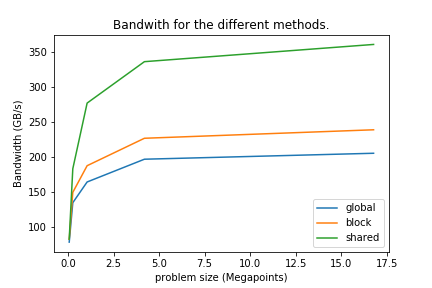
\includegraphics{3-1.png}\\
 	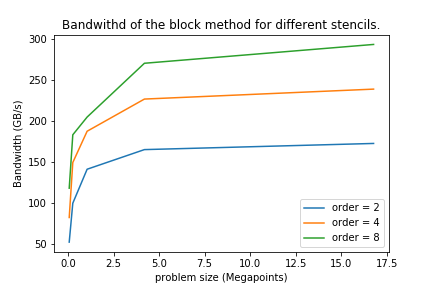
\includegraphics{3-2.png}\\
 	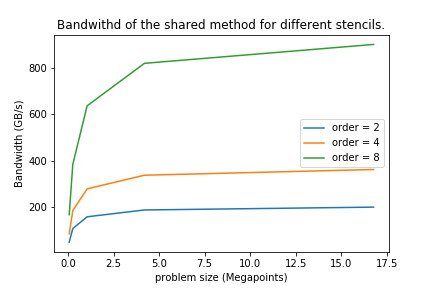
\includegraphics{3-3.png}
 	\section*{Question 4}
 	Except for the smallest grid size the performance in order from worst to best is global, block and shared. For the lowest grid size not all the resources cannot be utilized simultaneously, to the idle time as a fraction of the total time will be larger. This is why the different methods perform the same for the smaller grid sizes. The higher order methods perform better than the lower order ones due to the memory copying needed to for a single mesh point. Because any memory request will copy an entire cache line no matter how many elements are actually used. The higher order methods will use more of the elements in the row of the stencil, which is coalesced in memory, and therefore make more efficient use of cache lines. Since the bandwidth calculation depends on stencil size the bandwidth will increase for higher order methods.\\
 	The block method will perform better than the global method because the there is less memory traffic in total. In the global method each thread will request the memory for its operation after which the allocted memory in the cache may dissapear. In the block method one thread will perform multiple operations. This keeps the requested memory in the cache for longer which will make access to it faster for the thread and other threads in the warp. This is the same reason why the shared method performs best. In this method all the memory required by a single block is stored locally and remains there until the block is finished. This significantly reduces the memory traffic and explains why the shared memory so much faster.
 \end{document}